\section{Documentation}

Source code alone is not enough to document larger projects. Developers need additional information, such as possible results or side effects of a method, and consistency conditions of data structures. Therefore documentation is key to ensure that software is reliable and maintainable over time.

\subsection{What to document}

There are two stakeholders, clients and implementors. For clients it is important to document the interface, how to use the code. For stakeholders it is important to document how the code works. For the clients document the methods and constructors that can be used to interact with the software, as well as any preconditions and postconditions that must be met. For implementors, documentation should include the algorithms and data structures used in the software, as well as any invariants and assertions that must be maintained.

\subsection{How to document}

Documentation does not only consist of comments. Using type annotations, modifiers, assertions and effect systems can also be considered documentation. Still, comments are a large part of good documentation. They provide simple, flexible way of documenting interfaces and implementations. A good documentation using comments can look as follows:

\begin{center}
	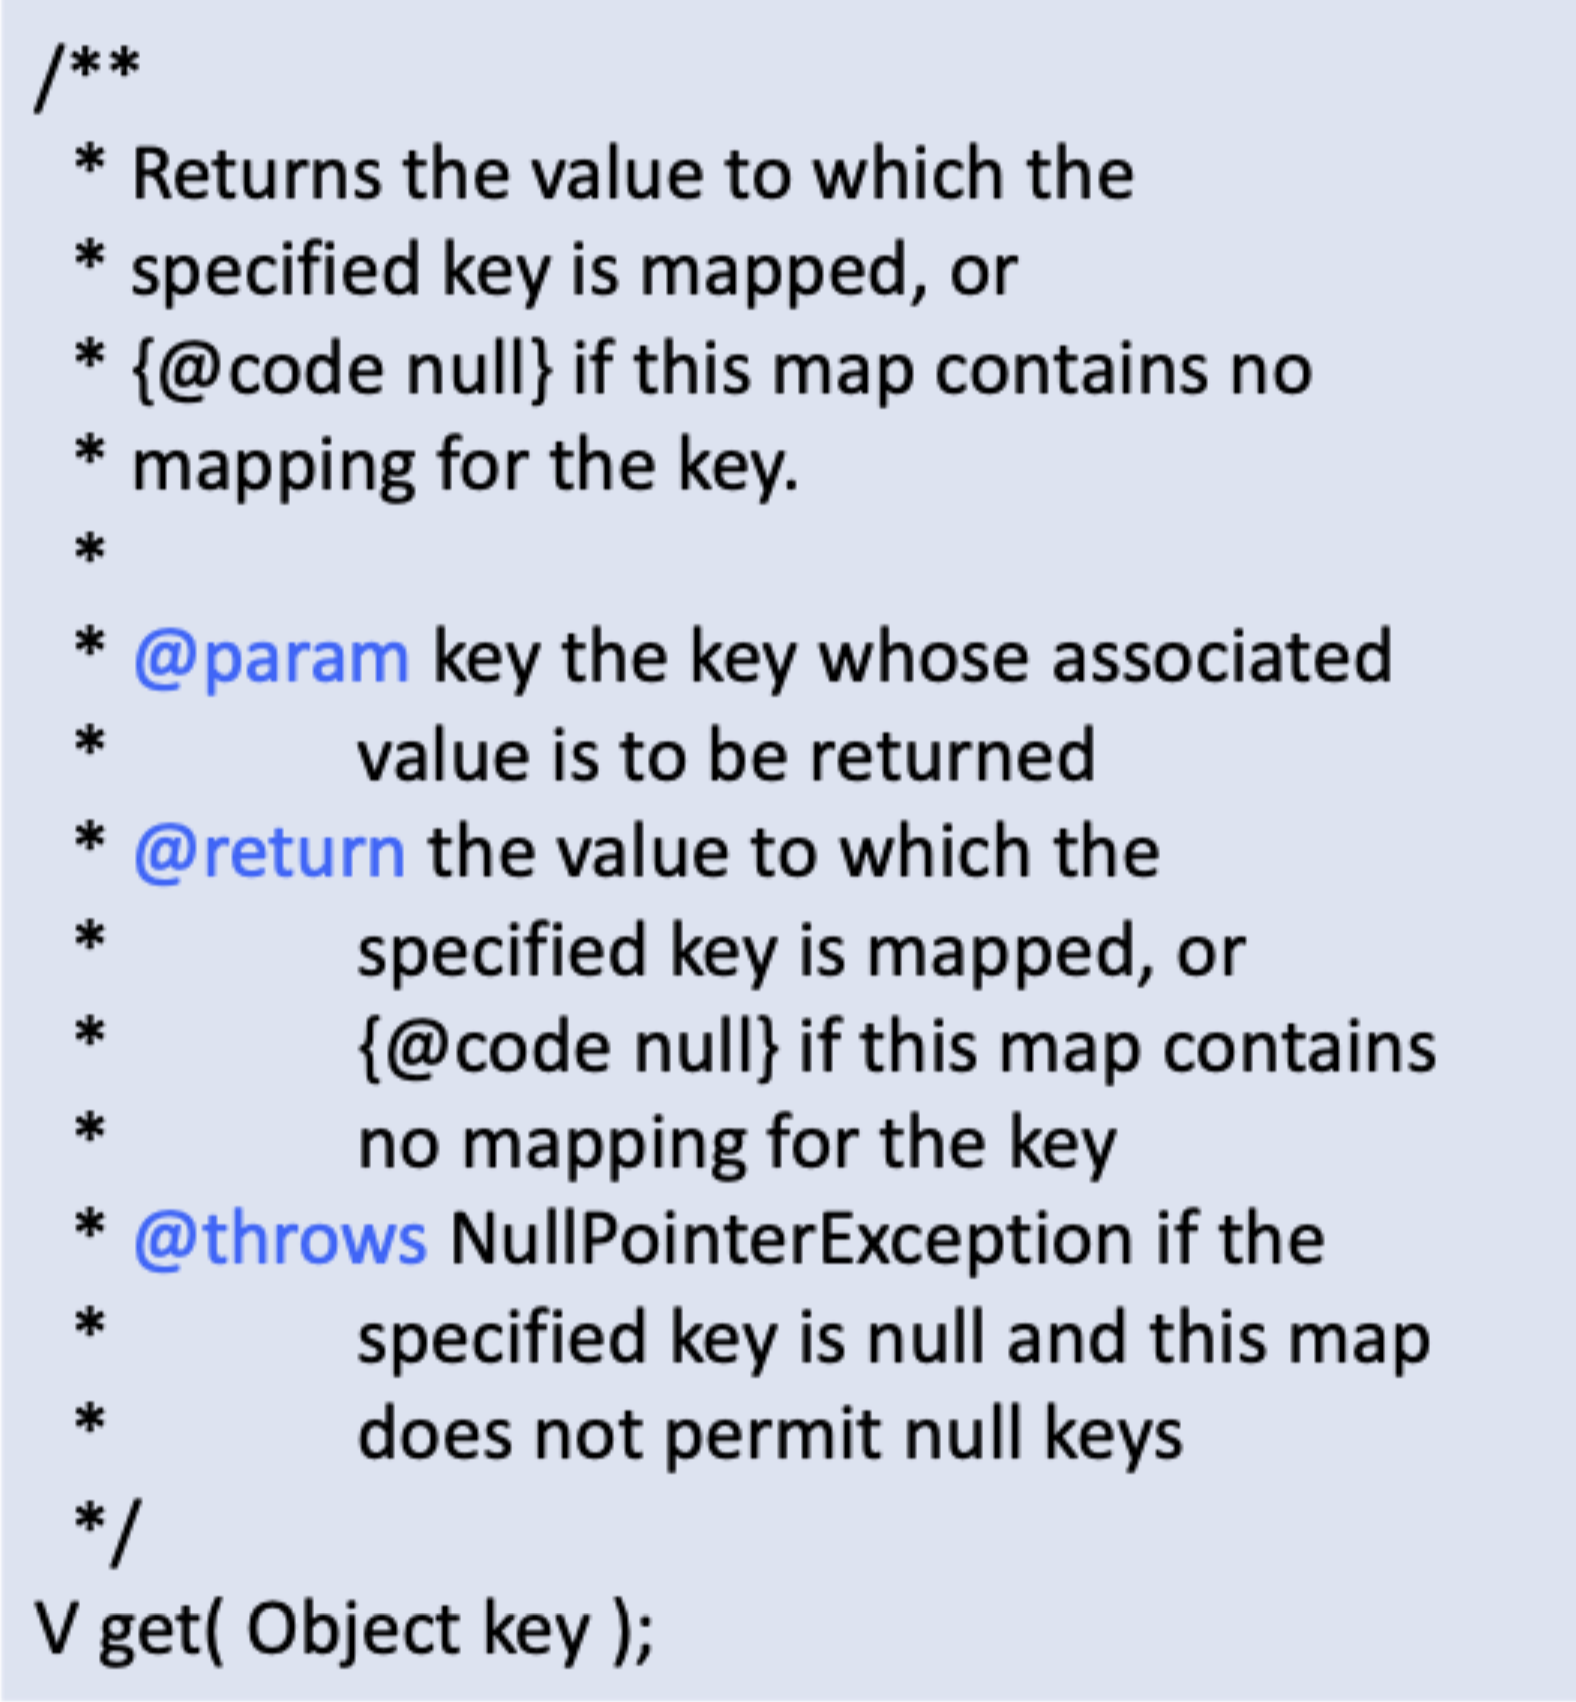
\includegraphics[width=0.5\columnwidth]{assets/comment}
\end{center}

Using diagrams and examples to illustrate complex concepts can further help to make the documentation easier to understand. Consistent formatting and naming conventions can further improve the documentation. Finally, regular reviews and updates ensure that it remains accurate and up-to-date.